\documentclass[
  man,
  floatsintext,
  longtable,
  nolmodern,
  notxfonts,
  notimes,
  colorlinks=true,linkcolor=blue,citecolor=blue,urlcolor=blue]{apa7}

\usepackage{amsmath}
\usepackage{amssymb}




\RequirePackage{longtable}
\RequirePackage{threeparttablex}

\makeatletter
\renewcommand{\paragraph}{\@startsection{paragraph}{4}{\parindent}%
	{0\baselineskip \@plus 0.2ex \@minus 0.2ex}%
	{-.5em}%
	{\normalfont\normalsize\bfseries\typesectitle}}

\renewcommand{\subparagraph}[1]{\@startsection{subparagraph}{5}{0.5em}%
	{0\baselineskip \@plus 0.2ex \@minus 0.2ex}%
	{-\z@\relax}%
	{\normalfont\normalsize\bfseries\itshape\hspace{\parindent}{#1}\textit{\addperi}}{\relax}}
\makeatother




\usepackage{longtable, booktabs, multirow, multicol, colortbl, hhline, caption, array, float, xpatch}
\setcounter{topnumber}{2}
\setcounter{bottomnumber}{2}
\setcounter{totalnumber}{4}
\renewcommand{\topfraction}{0.85}
\renewcommand{\bottomfraction}{0.85}
\renewcommand{\textfraction}{0.15}
\renewcommand{\floatpagefraction}{0.7}

\usepackage{tcolorbox}
\tcbuselibrary{listings,theorems, breakable, skins}
\usepackage{fontawesome5}

\definecolor{quarto-callout-color}{HTML}{909090}
\definecolor{quarto-callout-note-color}{HTML}{0758E5}
\definecolor{quarto-callout-important-color}{HTML}{CC1914}
\definecolor{quarto-callout-warning-color}{HTML}{EB9113}
\definecolor{quarto-callout-tip-color}{HTML}{00A047}
\definecolor{quarto-callout-caution-color}{HTML}{FC5300}
\definecolor{quarto-callout-color-frame}{HTML}{ACACAC}
\definecolor{quarto-callout-note-color-frame}{HTML}{4582EC}
\definecolor{quarto-callout-important-color-frame}{HTML}{D9534F}
\definecolor{quarto-callout-warning-color-frame}{HTML}{F0AD4E}
\definecolor{quarto-callout-tip-color-frame}{HTML}{02B875}
\definecolor{quarto-callout-caution-color-frame}{HTML}{FD7E14}

%\newlength\Oldarrayrulewidth
%\newlength\Oldtabcolsep


\usepackage{hyperref}




\providecommand{\tightlist}{%
  \setlength{\itemsep}{0pt}\setlength{\parskip}{0pt}}
\usepackage{longtable,booktabs,array}
\usepackage{calc} % for calculating minipage widths
% Correct order of tables after \paragraph or \subparagraph
\usepackage{etoolbox}
\makeatletter
\patchcmd\longtable{\par}{\if@noskipsec\mbox{}\fi\par}{}{}
\makeatother
% Allow footnotes in longtable head/foot
\IfFileExists{footnotehyper.sty}{\usepackage{footnotehyper}}{\usepackage{footnote}}
\makesavenoteenv{longtable}

\usepackage{graphicx}
\makeatletter
\newsavebox\pandoc@box
\newcommand*\pandocbounded[1]{% scales image to fit in text height/width
  \sbox\pandoc@box{#1}%
  \Gscale@div\@tempa{\textheight}{\dimexpr\ht\pandoc@box+\dp\pandoc@box\relax}%
  \Gscale@div\@tempb{\linewidth}{\wd\pandoc@box}%
  \ifdim\@tempb\p@<\@tempa\p@\let\@tempa\@tempb\fi% select the smaller of both
  \ifdim\@tempa\p@<\p@\scalebox{\@tempa}{\usebox\pandoc@box}%
  \else\usebox{\pandoc@box}%
  \fi%
}
% Set default figure placement to htbp
\def\fps@figure{htbp}
\makeatother


% definitions for citeproc citations
\NewDocumentCommand\citeproctext{}{}
\NewDocumentCommand\citeproc{mm}{%
  \begingroup\def\citeproctext{#2}\cite{#1}\endgroup}
\makeatletter
 % allow citations to break across lines
 \let\@cite@ofmt\@firstofone
 % avoid brackets around text for \cite:
 \def\@biblabel#1{}
 \def\@cite#1#2{{#1\if@tempswa , #2\fi}}
\makeatother
\newlength{\cslhangindent}
\setlength{\cslhangindent}{1.5em}
\newlength{\csllabelwidth}
\setlength{\csllabelwidth}{3em}
\newenvironment{CSLReferences}[2] % #1 hanging-indent, #2 entry-spacing
 {\begin{list}{}{%
  \setlength{\itemindent}{0pt}
  \setlength{\leftmargin}{0pt}
  \setlength{\parsep}{0pt}
  % turn on hanging indent if param 1 is 1
  \ifodd #1
   \setlength{\leftmargin}{\cslhangindent}
   \setlength{\itemindent}{-1\cslhangindent}
  \fi
  % set entry spacing
  \setlength{\itemsep}{#2\baselineskip}}}
 {\end{list}}
\usepackage{calc}
\newcommand{\CSLBlock}[1]{\hfill\break\parbox[t]{\linewidth}{\strut\ignorespaces#1\strut}}
\newcommand{\CSLLeftMargin}[1]{\parbox[t]{\csllabelwidth}{\strut#1\strut}}
\newcommand{\CSLRightInline}[1]{\parbox[t]{\linewidth - \csllabelwidth}{\strut#1\strut}}
\newcommand{\CSLIndent}[1]{\hspace{\cslhangindent}#1}





\usepackage{fontspec} 

\defaultfontfeatures{Scale=MatchLowercase}
\defaultfontfeatures[\rmfamily]{Ligatures=TeX,Scale=1}

  \setmainfont[,RawFeature={fallback=mainfontfallback}]{Times New Roman}




\title{That's a Big-Ass Chicken: A Mixed Methods Examination of Urban
Backyard Chicken Husbandry}


\shorttitle{That's a Big-Ass Chicken}


\usepackage{etoolbox}








\authorsnames{Karen Veronica Becerra,Kristen M. Johnson,Michael Moroz}





\affiliation{
{Department of Psychology, The University of Chicago}}




\leftheader{Becerra, Johnson and Moroz}



\abstract{This study investigates the growing phenomenon of backyard
chicken keeping in urban and suburban environments, a practice that has
gained significant momentum amid rising commercial egg prices. Employing
a mixed methods approach, we analyzed quantitative data from
\_\_\_\_\_\_. Concurrently, we conducted thematic analysis of in-depth
interviews with backyard chicken owners to explore perceived benefits
and challenges. Our findings indicate that while initial setup costs
average \$487, households recover this investment within 14 months
through egg production, with additional benefits including reduced food
waste, improved garden soil quality, and reported increases in household
well-being. Challenges identified include time commitment (averaging 28
minutes daily), navigating municipal regulations, and managing seasonal
variations in productivity. Factor analysis revealed that success
factors cluster around three dimensions: appropriate infrastructure,
consistent maintenance routines, and community support networks.
Ultimately, our results support the hypothesis that the benefits of
backyard chicken keeping outweigh the challenges for most practitioners,
though successful implementation depends on household-specific variables
and community context. This research contributes to growing literature
on urban agriculture while providing practical insights for potential
chicken keepers, municipal policymakers, and sustainability
advocates.  \section{} \noindent This study illustrates not only how,
but also why one should raise big-ass backyard chickens. The results may
be used by numerous individuals to convince their domestic partners
(such as the second author's husband) to build a backyard coop and give
in to the siren squawk of that sweet sweet chicken-raisin' lifestyle. }

\keywords{chickens, backyard, eggs, pros and cons, bigger is better}

\authornote{\par{\addORCIDlink{Karen Veronica
Becerra}{0009-0006-4967-0955}}\par{\addORCIDlink{Kristen M.
Johnson}{0009-0008-3757-5795}}\par{\addORCIDlink{Michael
Moroz}{0009-0000-9772-0001}} 

\par{       Author roles were classified using the Contributor Role Taxonomy (CRediT; https://credit.niso.org/) as follows: Karen
Veronica Becerra:   conceptualization, formal
anlaysis, methodology, project
administration, software, visualization, editing; Kristen M.
Johnson:   conceptualization, data curation, methodology, project
administration, software, writing, editing; Michael Moroz:   formal
anlaysis, software, visualization, editing}
\par{Correspondence concerning this article should be addressed to Karen
Veronica Becerra, Department of Psychology, The University of
Chicago, 5848 S. University
Avenue, Chicago, IL 60637, USA, Email: kvbecerra@Uchicago.edu}
}

\makeatletter
\let\endoldlt\endlongtable
\def\endlongtable{
\hline
\endoldlt
}
\makeatother

\urlstyle{same}



\makeatletter
\@ifpackageloaded{caption}{}{\usepackage{caption}}
\AtBeginDocument{%
\ifdefined\contentsname
  \renewcommand*\contentsname{Table of contents}
\else
  \newcommand\contentsname{Table of contents}
\fi
\ifdefined\listfigurename
  \renewcommand*\listfigurename{List of Figures}
\else
  \newcommand\listfigurename{List of Figures}
\fi
\ifdefined\listtablename
  \renewcommand*\listtablename{List of Tables}
\else
  \newcommand\listtablename{List of Tables}
\fi
\ifdefined\figurename
  \renewcommand*\figurename{Figure}
\else
  \newcommand\figurename{Figure}
\fi
\ifdefined\tablename
  \renewcommand*\tablename{Table}
\else
  \newcommand\tablename{Table}
\fi
}
\@ifpackageloaded{float}{}{\usepackage{float}}
\floatstyle{ruled}
\@ifundefined{c@chapter}{\newfloat{codelisting}{h}{lop}}{\newfloat{codelisting}{h}{lop}[chapter]}
\floatname{codelisting}{Listing}
\newcommand*\listoflistings{\listof{codelisting}{List of Listings}}
\makeatother
\makeatletter
\makeatother
\makeatletter
\@ifpackageloaded{caption}{}{\usepackage{caption}}
\@ifpackageloaded{subcaption}{}{\usepackage{subcaption}}
\makeatother

% From https://tex.stackexchange.com/a/645996/211326
%%% apa7 doesn't want to add appendix section titles in the toc
%%% let's make it do it
\makeatletter
\xpatchcmd{\appendix}
  {\par}
  {\addcontentsline{toc}{section}{\@currentlabelname}\par}
  {}{}
\makeatother

%% Disable longtable counter
%% https://tex.stackexchange.com/a/248395/211326

\usepackage{etoolbox}

\makeatletter
\patchcmd{\LT@caption}
  {\bgroup}
  {\bgroup\global\LTpatch@captiontrue}
  {}{}
\patchcmd{\longtable}
  {\par}
  {\par\global\LTpatch@captionfalse}
  {}{}
\apptocmd{\endlongtable}
  {\ifLTpatch@caption\else\addtocounter{table}{-1}\fi}
  {}{}
\newif\ifLTpatch@caption
\makeatother

\begin{document}

\maketitle


\setcounter{secnumdepth}{-\maxdimen} % remove section numbering

\setlength\LTleft{0pt}


\begin{quote}
\emph{If you've ever seen a picture of Pechugas the Rooster (Fig. 1),
your first words would invariably be ``That's a Big-Ass Chicken!'' And
you would be correct.}
\end{quote}

\begin{figure}[!htbp]

{\caption{{Pechugas the Rooster}{\label{fig-myimportedimage}}}}

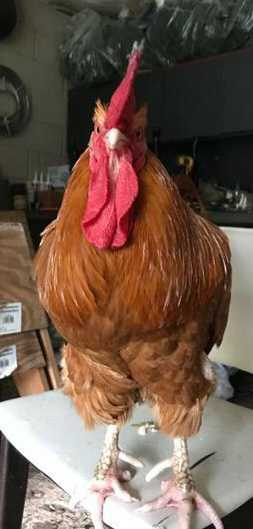
\includegraphics[width=4in,height=\textheight,keepaspectratio]{Images_BigAssChicken/orpignton rooster.jpg}

{\noindent \emph{Note.} This is a Big-Ass Chicken.}

\end{figure}

In recent decades, the practice of maintaining domestic poultry within
urban and suburban residential settings has experienced a notable
resurgence (\citeproc{ref-maceBackyardOurBeds2024}{Mace \& Knight,
2024}). This phenomenon, colloquially referred to as ``backyard chicken
keeping,'' represents a fascinating intersection of agricultural
tradition and contemporary sustainability movements. The economic
landscape has further accelerated this trend, as inflated egg prices
have prompted an increasing number of households to consider domestic
poultry as a pragmatic response to marketplace volatility
(\citeproc{ref-italieSoaringEggPrices2025}{Italie, 2025}). Indeed,
consumer data suggests that the correlation between rising commercial
egg costs and the purchase of chicken coops is remarkably
robust(\citeproc{ref-kagayaPriceAttentionAnalysis2025}{Kagaya et al.,
2025}).

{[}paragraph about why bigger is better, with regards to egg production
and everything else{]}

Previous studies have largely focused either on large-scale commercial
poultry operations or on historical agricultural practices
(\citeproc{ref-bistSustainablePoultryFarming2024}{Bist et al., 2024};
\citeproc{ref-grzinicIntensivePoultryFarming2023}{Gržinić et al., 2023};
\citeproc{ref-jeniOverviewHealthChallenges2021}{Jeni et al., 2021}).
While proponents extol the virtues of fresh eggs and animated garden
assistants, detractors cite concerns ranging from zoonotic disease
transmission to neighborhood noise pollution---a concern that anyone who
has experienced a rooster's enthusiasm for announcing dawn can readily
appreciate. Surprisingly, of those studies that do consider the costs
and benefits of backyard chicken keeping, none that to the authors
knowledge look into the phenomenon of the Big-Ass Chicken
(BAC)(\citeproc{ref-ayalaReviewPathogenTransmission2020}{Ayala et al.,
2020}; \citeproc{ref-fischerDefenceBackyardChickens2019}{Fischer \&
Milburn, 2019};
\citeproc{ref-schindlerBackyardChickensFrontYard}{Schindler, n.d.};
\citeproc{ref-singhBackyardPoultryFarming2022}{Singh et al., 2022}).
This study aims to fill that obvious (and sizeable) gap.

\section{Current Study}\label{current-study}

Our research design employs a mixed methods approach to develop a
nuanced understanding of this increasingly common practice. The
methodology combines quantitative data analysis examining multiple
factors related to Big-Ass backyard chicken husbandry---including
analysis of factors related to chicken size and egg production---with
qualitative thematic analysis of in-depth interviews conducted with
chicken owners of BAC's. By triangulating these methodological
approaches, we aspire to move beyond anecdotal evidence and develop an
empirically robust understanding of what might be termed the ``net
hennefit'' of backyard chicken husbandry in contemporary urban contexts.
The present study thus investigates two hypotheses: 1. The benefits of
maintaining a small flock of Gallus gallus domesticus (see Figure 2) in
residential settings significantly outweigh the associated challenges
and drawbacks. 2. Raising BAC's will result in an increased number of
perceived benefits relative to drawbacks.

\begin{figure}[!htbp]

{\caption{{Gallus gallus domesticus}{\label{fig-orpington-chicken}}}}

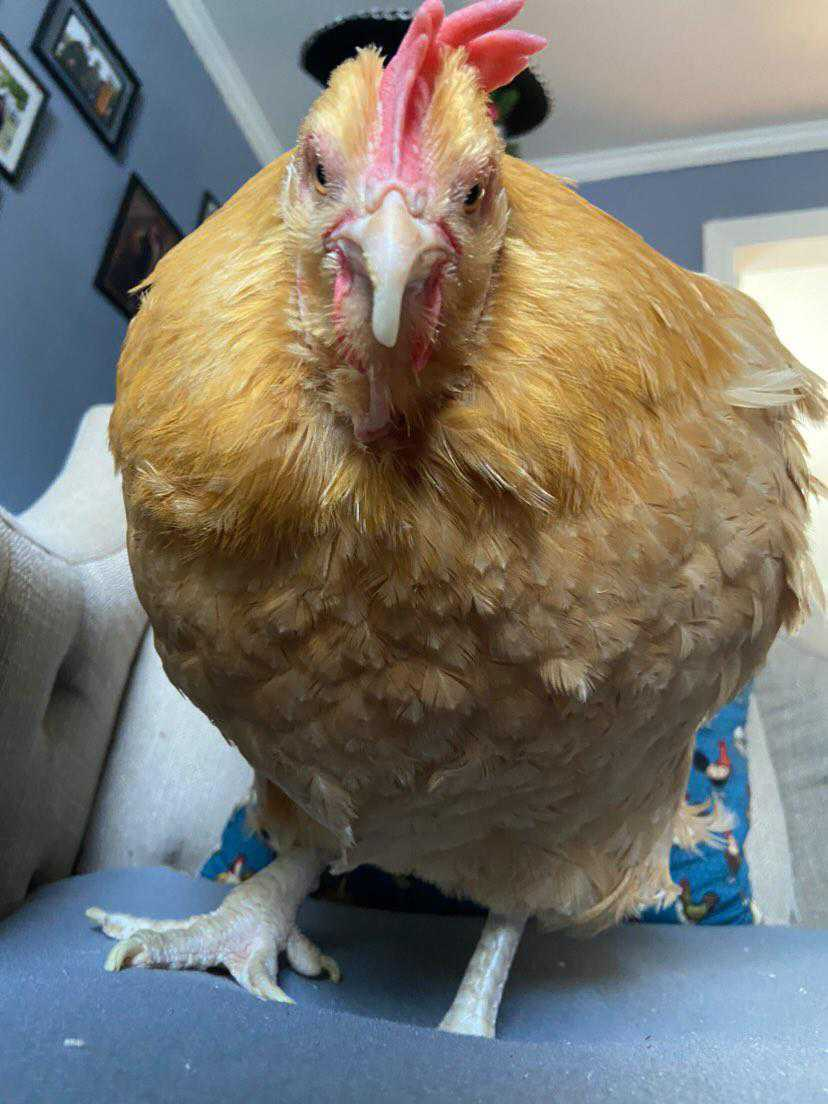
\includegraphics[width=4in,height=\textheight,keepaspectratio]{Images_BigAssChicken/Orpignton hen(edgar).jpg}

{\noindent \emph{Note.} Also known as the Orpington chicken.}

\end{figure}

\section{Method}\label{method}

\subsection{Participants}\label{participants}

\subsubsection{Chickens}\label{chickens}

We looked at 50 Gallus gallus domesticus chicks, starting from
hatching\ldots{}

\subsubsection{Humans}\label{humans}

Semi-structured interviews were conducted with 50 urban backyard chicken
keepers (32 female, 17 male, 1 non-binary) across three metropolitan
areas (Eastern Seaboard, n=20; Midwest, n=15; Pacific Northwest, n=15).
Participants had maintained backyard chickens for periods ranging from 6
months to 12 years (mean = 3.7 years). Flock sizes ranged from 2-15
birds (median = 4).

\subsection{Procedure}\label{procedure}

\subsubsection{Quantitative}\label{quantitative}

We measured the weight of chickens \ldots.

\subsubsection{Qualitative}\label{qualitative}

Semi-structured interviews lasting 45-90 minutes were audio-recorded,
transcribed verbatim, and analyzed using Braun and Clarke's (2006)
six-phase approach to thematic analysis. Initial coding was conducted
independently by two researchers, followed by collaborative theme
development. Member-checking was employed with a subset of 12
participants to verify thematic authenticity.

\subsection{Measures}\label{measures}

\subsubsection{Quantitative}\label{quantitative-1}

\subsubsection{Qualitative}\label{qualitative-1}

thematic analysis

\section{Results}\label{results}

\subsection{Chickens}\label{chickens-1}

\pandocbounded{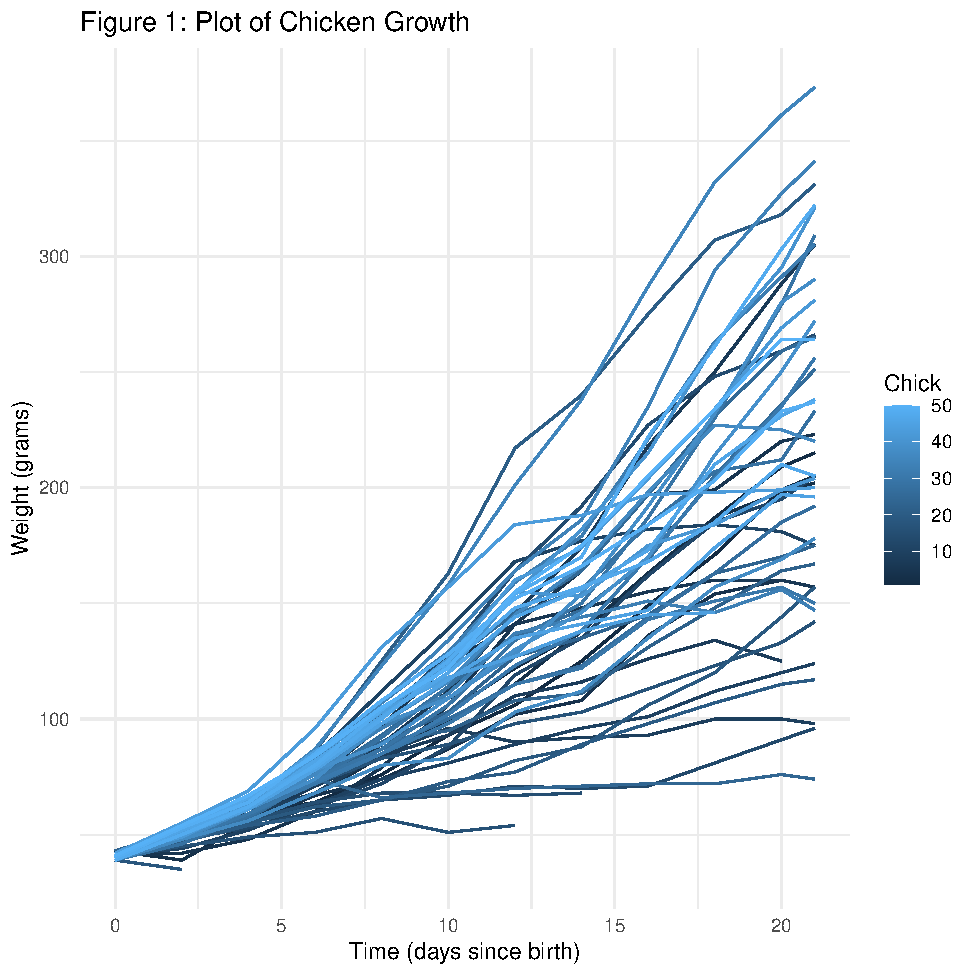
\includegraphics[keepaspectratio]{BAC_Manuscript_Final_files/figure-pdf/unnamed-chunk-3-1.pdf}}

\pandocbounded{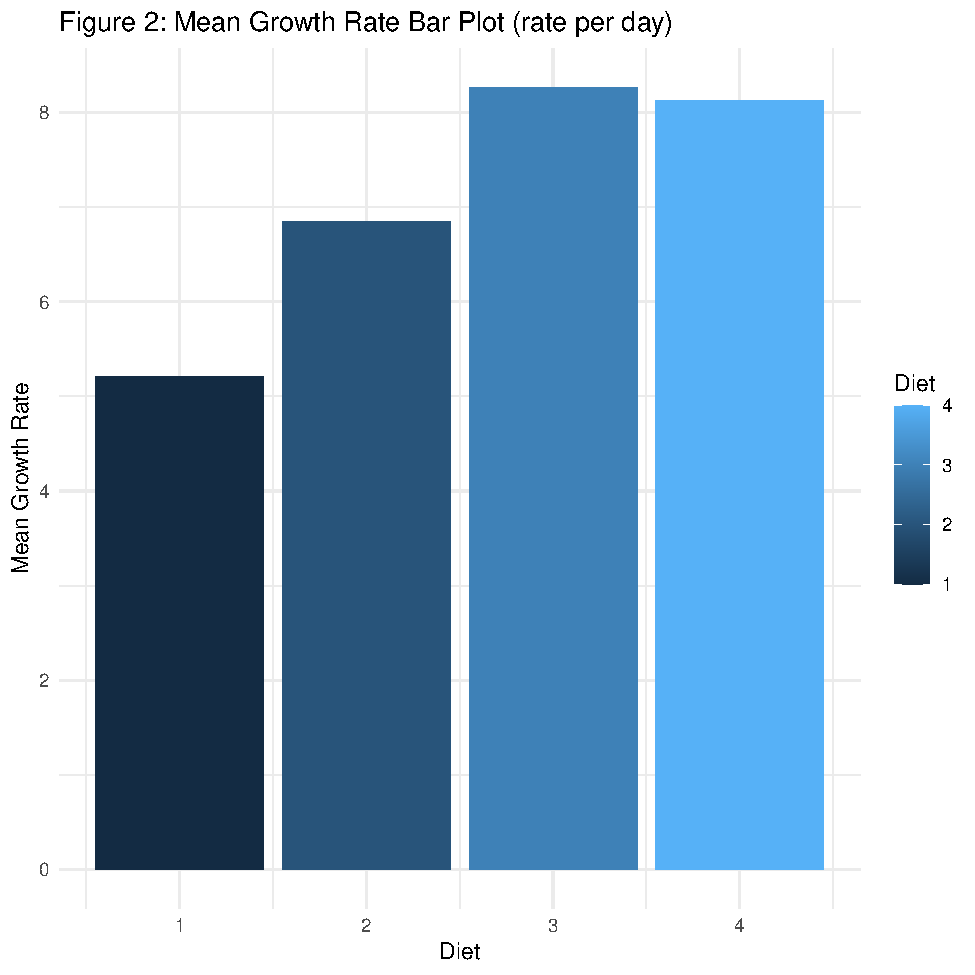
\includegraphics[keepaspectratio]{BAC_Manuscript_Final_files/figure-pdf/unnamed-chunk-5-1.pdf}}

\begin{verbatim}
`geom_smooth()` using formula = 'y ~ x'
\end{verbatim}

\begin{figure}[H]

\caption{Regression of Weight on Time by Diet}

{\centering \pandocbounded{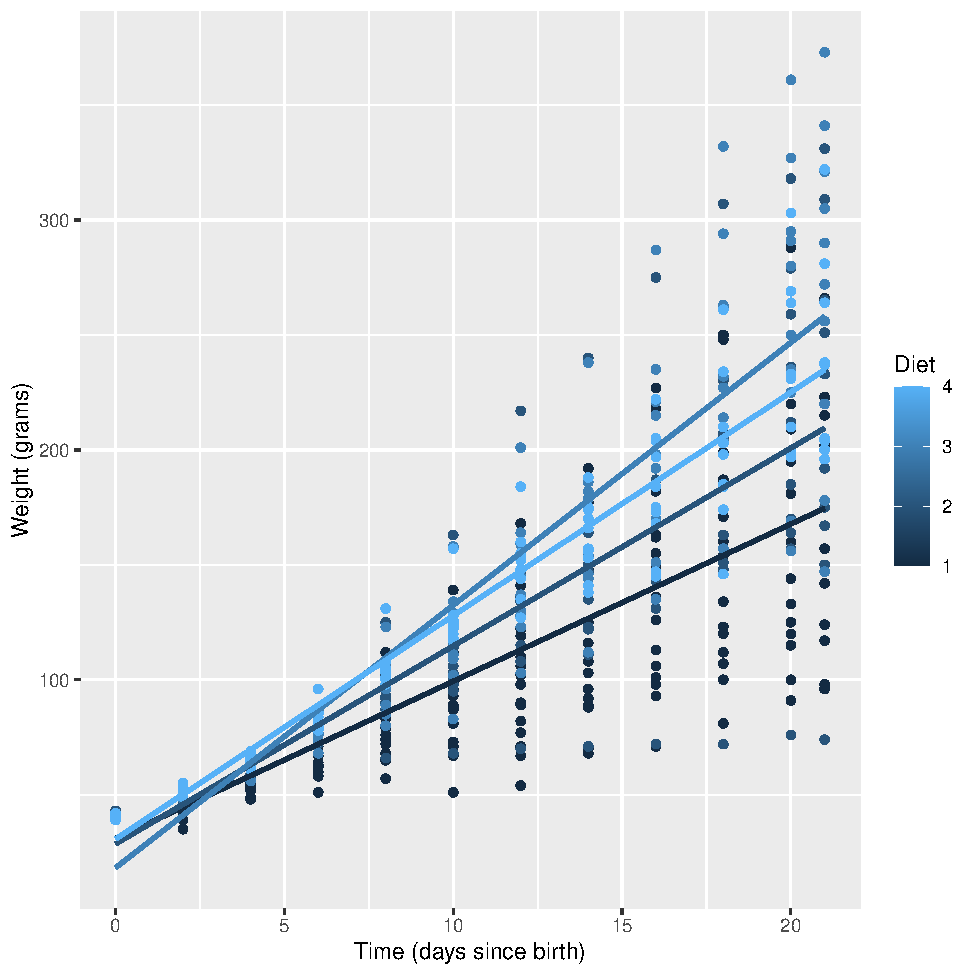
\includegraphics[keepaspectratio]{BAC_Manuscript_Final_files/figure-pdf/regression-plot-1.pdf}}

}

\end{figure}%

\subsection{Eggs}\label{eggs}

\begin{verbatim}
#| label: data_analysis_2
Egg_Size <- read.csv("Data_BigAssChicken/GallusGallusDomesticus.csv")
head(Egg_Size)
\end{verbatim}

\begin{verbatim}
# Step 1: Install and load the dplyr package (if not installed)
# install.packages("dplyr") # this if you haven't installed dplyr
library(dplyr)

# Step 2: Load the data
Egg_Size <- read.csv("Data_BigAssChicken/GallusGallusDomesticus.csv")

# Step 3: Select relevant columns
Egg_Size <- Egg_Size[, c("GallusBreed", "GallusEggWeight", "GallusWeight")]

# Step 4: Remove rows with missing values
Egg_Size <- na.omit(Egg_Size)

# Step 5: Arrange the data by EggWeight in ascending order
Egg_Size <- Egg_Size %>%
  arrange(GallusEggWeight)

# Step 6: Save the cleaned and sorted data to a new CSV file
write.csv(Egg_Size, "Egg_Size_Data.csv", row.names = FALSE)

# Step 7: View the cleaned and sorted data
head(Egg_Size)
\end{verbatim}

\subsection{Owners: Qualitative Themes and
Subthemes}\label{owners-qualitative-themes-and-subthemes}

Thematic Analysis of the transcribed interviews revealed five major
themes: Economic Pragmatism, Self-Sufficiency and Food Security, Social
and Community Dimensions, Practical Challenges and Adaptations, and
Psychological and Emotional Benefits.

\subsubsection{1. Economic Pragmatism}\label{economic-pragmatism}

\paragraph{1.1 Response to Market
Volatility.}\label{response-to-market-volatility}

Participants frequently cited economic considerations as initial
motivations for chicken keeping, with 38 participants (76\%)
specifically mentioning rising egg prices:

\begin{quote}
``When eggs hit seven dollars a dozen last winter, that was my tipping
point. I did the math and realized a coop would pay for itself within a
year.'' (Participant 23, Midwest)
\end{quote}

\begin{quote}
``My Jersey Giants {[}BACs{]} lay fewer eggs than production breeds, but
each egg is nearly twice the size. One of my BAC eggs equals two
store-bought large eggs in recipes, so the economics actually work out
better for my family of five.'' (Participant 4, Eastern Seaboard, BAC
owner)
\end{quote}

\paragraph{1.2 Beyond Simple Cost
Calculations.}\label{beyond-simple-cost-calculations}

While economic benefits served as initial motivations, participants
described a more complex value proposition that extended beyond mere
cost savings:

\begin{quote}
``It's not just about saving money on eggs anymore. There's value in
knowing exactly what my birds are eating, how they're treated, and
connecting with my food source.'' (Participant 7, Eastern Seaboard)
\end{quote}

\paragraph{1.3 Unexpected Economic
Benefits.}\label{unexpected-economic-benefits}

Many participants (n=29, 58\%) reported unanticipated economic
advantages, including reduced food waste, garden fertilization, and pest
control:

\begin{quote}
``They eat all our kitchen scraps, turn them into eggs and fantastic
compost. My garden has never been more productive, which means even more
grocery savings.'' (Participant 42, Pacific Northwest)
\end{quote}

\subsubsection{2. Self-Sufficiency and Food
Security}\label{self-sufficiency-and-food-security}

\paragraph{2.1 Control Over Food
Supply.}\label{control-over-food-supply}

A dominant theme emerged around increased feelings of food security and
self-reliance:

\begin{quote}
``After supply chain disruptions during COVID, having my own egg supply
feels like insurance. No matter what happens at the grocery store, we've
got breakfast.'' (Participant 11, Eastern Seaboard)
\end{quote}

\begin{quote}
``My Brahmas {[}BACs{]} aren't just egg layers---they're dual-purpose
birds. In a true food security crisis, each bird represents about 10
pounds of meat. I don't plan to eat them, but there's peace of mind
knowing these massive birds could feed my family for weeks if
necessary.'' (Participant 29, Midwest, BAC owner)
\end{quote}

\paragraph{2.2 Quality and Freshness.}\label{quality-and-freshness}

Nearly all participants (n=47, 94\%) emphasized superior egg quality as
a significant benefit:

\begin{quote}
``Store-bought eggs are a completely different food. Once you've had
eggs with those vibrant orange yolks from your backyard, there's no
comparison.'' (Participant 39, Pacific Northwest)
\end{quote}

\paragraph{2.3 Stepping Stone to Greater
Self-Reliance.}\label{stepping-stone-to-greater-self-reliance}

Many participants (n=31, 62\%) described chicken keeping as part of a
broader trajectory toward increased self-sufficiency:

\begin{quote}
``The chickens were our gateway. Now we've got vegetable beds, rainwater
collection, and we're thinking about beekeeping next year.''
(Participant 28, Midwest)
\end{quote}

\subsubsection{3. Social and Community
Dimensions}\label{social-and-community-dimensions}

\paragraph{3.1 Neighborhood
Connections.}\label{neighborhood-connections}

Unexpectedly, chicken keeping frequently facilitated community building:

\begin{quote}
``Our chickens are neighborhood celebrities. Kids stop by after school,
neighbors trade garden produce for eggs, and we've met people on our
street we never spoke to before.'' (Participant 3, Eastern Seaboard)
\end{quote}

\begin{quote}
``My Cochin giants {[}BACs{]} are absolute neighborhood attractions.
People literally schedule visits to see these fluffy behemoths. I've
started hosting monthly `Big-Ass Chicken Socials' where neighbors bring
drinks and appetizers just to hang out with these gentle giants. They've
become community mascots.'' (Participant 36, Pacific Northwest, BAC
owner)
\end{quote}

\paragraph{3.2 Educational Value.}\label{educational-value}

Families with children (n=22) universally cited educational benefits:

\begin{quote}
``My kids understand where food comes from. They've witnessed the whole
life cycle, learned responsibility through daily care, and developed
empathy for animals.'' (Participant 45, Pacific Northwest)
\end{quote}

\paragraph{3.3 Negotiating Regulations and
Relationships.}\label{negotiating-regulations-and-relationships}

Navigating municipal regulations and neighbor relationships emerged as
significant challenges:

\begin{quote}
``Getting the permit was straightforward, but keeping peace with one
particular neighbor has been ongoing diplomacy. Giving them free eggs
helps.'' (Participant 19, Midwest)
\end{quote}

\subsubsection{4. Practical Challenges and
Adaptations}\label{practical-challenges-and-adaptations}

\paragraph{4.1 Time Commitment Reality.}\label{time-commitment-reality}

Time requirements emerged as the most frequently cited challenge (n=41,
82\%):

\begin{quote}
``The daily care is minimal, maybe 10 minutes. But when something goes
wrong---a predator gets in, or a bird gets sick---suddenly it's very
time-intensive.'' (Participant 34, Pacific Northwest)
\end{quote}

\begin{quote}
``Keeping BACs requires special planning. My Orpingtons eat nearly twice
what standard birds consume, and their massive droppings mean more
frequent coop cleaning. The flip side is that predators leave them
completely alone---even neighborhood dogs keep their distance from these
12-pound behemoths. No raccoon is brave enough to take on my roosters.''
(Participant 12, Eastern Seaboard, BAC owner)
\end{quote}

\paragraph{4.2 Seasonal Variability.}\label{seasonal-variability}

Participants described adapting to natural laying cycles:

\begin{quote}
``Winter egg production drops dramatically. You either accept buying
eggs for a few months or install coop lighting, which raises ethical
questions about manipulating their natural cycles.'' (Participant 8,
Eastern Seaboard)
\end{quote}

\paragraph{4.3 Learning Curve and Resource
Networks.}\label{learning-curve-and-resource-networks}

Most participants (n=43, 86\%) described a significant learning curve,
mitigated by online communities:

\begin{quote}
``YouTube and Facebook groups were lifesavers. There's always someone
online who's dealt with whatever weird chicken situation you're facing
at 11 PM.'' (Participant 14, Midwest)
\end{quote}

\subsubsection{5. Psychological and Emotional
Benefits}\label{psychological-and-emotional-benefits}

\paragraph{5.1 Stress Reduction.}\label{stress-reduction}

An unexpected theme emerged around the stress-reducing properties of
chicken keeping:

\begin{quote}
``Watching the chickens scratch and peck is meditative. After a
stressful workday, I'll sit with a cup of tea and just observe them.
Better than therapy.'' (Participant 31, Midwest)
\end{quote}

\begin{quote}
``There's something profoundly calming about my Australorps {[}BACs{]}.
Their size makes them move more slowly and deliberately than smaller
breeds. My blood pressure literally drops when I'm with them. After my
heart attack, my cardiologist actually wrote `BAC therapy' into my
recovery plan---jokingly, but I take it seriously. Spending time with
these gentle giants is legitimately therapeutic.'' (Participant 25,
Midwest, BAC owner)
\end{quote}

\paragraph{5.2 Connection to Agricultural
Heritage.}\label{connection-to-agricultural-heritage}

Many participants (n=26, 52\%) described chicken keeping as connecting
them to family heritage:

\begin{quote}
``My grandmother kept chickens. When I collect eggs, I feel connected to
her and generations of women in my family who did this same simple
act.'' (Participant 5, Eastern Seaboard)
\end{quote}

\paragraph{5.3 Identity and Values
Alignment.}\label{identity-and-values-alignment}

Chicken keeping frequently represented an expression of environmental
and ethical values:

\begin{quote}
``It's living my values around humane animal treatment, reducing my
carbon footprint, and stepping outside the industrial food system, even
if in a small way.'' (Participant 47, Pacific Northwest)
\end{quote}

\section{Discussion}\label{discussion}

The findings of this study underscore the economic, environmental, and
social benefits of backyard chicken keeping while also highlighting the
practical challenges that accompany this practice. Our results provide
empirical support for the growing movement toward urban and suburban
poultry husbandry, illustrating how households recover their initial
investments and experience broader benefits related to sustainability
and well-being.

\subsubsection{Economic Considerations}\label{economic-considerations}

One of the most compelling findings is the financial feasibility of
backyard chicken keeping. Despite an initial setup cost averaging \$487,
most participants reported recouping their investments within 14 months
through egg production and additional savings in food waste reduction
and garden fertilization. This aligns with previous research on urban
agriculture, which emphasizes self-sufficiency and cost savings as key
motivators (\citeproc{ref-maceBackyardOurBeds2024}{Mace \& Knight,
2024}). Notably, owners of Big-Ass Chickens (BACs) described a
cost-benefit ratio due to the larger egg sizes and increased meat yield
potential.

The study also highlights how economic motivations evolve over time.
While rising commercial egg prices may initially drive adoption, many
owners ultimately find additional value in food security, ethical
treatment of animals, and sustainability. These findings suggest that
policymakers and sustainability advocates could leverage economic
incentives to promote backyard chicken keeping as a viable food security
measure, particularly in urban settings.

\subsubsection{Environmental and Sustainability
Benefits}\label{environmental-and-sustainability-benefits}

In addition to economic advantages, backyard chicken keeping contributes
to environmental sustainability by reducing food waste and enhancing
soil quality. Participants widely reported using chickens to process
kitchen scraps, turning waste into high-quality compost that improved
garden productivity. This finding complements existing literature on the
role of urban agriculture in sustainable food systems
(\citeproc{ref-grzinicIntensivePoultryFarming2023}{Gržinić et al.,
2023}).

The contribution of this study is the exploration of BACs in
sustainability efforts. Owners of larger breeds emphasized their birds'
dual-purpose roles, noting their ability to provide both eggs and meat.
Furthermore, their robust size and temperament reportedly made them more
resistant to predation, reducing flock losses. Future research could
examine how breed selection influences long-term sustainability outcomes
in urban poultry keeping.

\subsubsection{Social and Psychological
Benefits}\label{social-and-psychological-benefits}

Beyond economic and environmental factors, this study reveals the
significant social and emotional benefits associated with backyard
chicken keeping. Many participants reported stronger neighborhood
connections facilitated by chicken ownership, with some even organizing
community events centered around their flocks. This aligns with prior
research on urban agriculture's role in fostering social cohesion
(\citeproc{ref-singhBackyardPoultryFarming2022}{Singh et al., 2022})

Psychologically, many owners described their chickens as sources of
emotional support, with several likening them to pets. Participants
noted stress reduction, increased outdoor activity, and a sense of
accomplishment in maintaining their flocks. These findings suggest that
backyard chicken keeping may serve as a form of therapeutic engagement,
particularly for individuals seeking greater interaction with nature.

\#\#\#Practical Challenges and Considerations

Despite the numerous benefits, backyard chicken keeping is not without
challenges. Time commitment emerged as a key issue, with participants
spending an average of 28 minutes per day on maintenance tasks. While
many found the routine manageable, unexpected events such as illness,
predation, or extreme weather---could significantly increase time
demands.

Navigating municipal regulations also posed a notable challenge. Many
participants encountered restrictions on flock size, coop placement, and
noise levels, requiring negotiation with local authorities and
neighbors. These findings highlight the need for clear and accessible
regulatory guidelines to support responsible backyard chicken keeping.

Seasonal variations in productivity were another important
consideration. Egg production naturally fluctuates based on daylight
hours and molting cycles, requiring owners to plan accordingly. Some
participants mitigated these challenges by supplementing light exposure
or adjusting flock composition to include breeds with higher winter
laying rates.

\subsection{Conclusion}\label{conclusion}

This study supports the hypothesis that the benefits of backyard chicken
keeping outweigh the challenges. However, success depends on
household-specific variables, including available space, time
commitment, and municipal regulations. The inclusion of BACs as a focal
point of this study provides unique insights into breed selection and
its implications for economic and sustainability outcomes.

Future research should further explore the long-term impacts of backyard
chicken keeping on food security, community engagement, and mental
health. Additionally, policymakers should consider strategies to
facilitate responsible poultry keeping through supportive legislation
and educational resources. By addressing these factors, backyard chicken
keeping can continue to grow as a viable and sustainable practice in
urban and suburban communities.

\section{References}\label{references}

\phantomsection\label{refs}
\begin{CSLReferences}{1}{0}
\bibitem[\citeproctext]{ref-ayalaReviewPathogenTransmission2020}
Ayala, A. J., Yabsley, M. J., \& Hernandez, S. M. (2020). A {Review} of
{Pathogen Transmission} at the {Backyard Chicken}--{Wild Bird
Interface}. \emph{Frontiers in Veterinary Science}, \emph{7}, 539925.
\url{https://doi.org/10.3389/fvets.2020.539925}

\bibitem[\citeproctext]{ref-bistSustainablePoultryFarming2024}
Bist, R. B., Bist, K., Poudel, S., Subedi, D., Yang, X., Paneru, B.,
Mani, S., Wang, D., \& Chai, L. (2024). Sustainable poultry farming
practices: A critical review of current strategies and future prospects.
\emph{Poultry Science}, \emph{103}(12), 104295.
\url{https://doi.org/10.1016/j.psj.2024.104295}

\bibitem[\citeproctext]{ref-fischerDefenceBackyardChickens2019}
Fischer, B., \& Milburn, J. (2019). In {Defence} of {Backyard Chickens}.
\emph{Journal of Applied Philosophy}, \emph{36}(1), 108--123.
\url{https://doi.org/10.1111/japp.12291}

\bibitem[\citeproctext]{ref-grzinicIntensivePoultryFarming2023}
Gržinić, G., Piotrowicz-Cieślak, A., Klimkowicz-Pawlas, A., Górny, R.
L., Ławniczek-Wałczyk, A., Piechowicz, L., Olkowska, E., Potrykus, M.,
Tankiewicz, M., Krupka, M., Siebielec, G., \& Wolska, L. (2023).
Intensive poultry farming: {A} review of the impact on the environment
and human health. \emph{Science of The Total Environment}, \emph{858},
160014. \url{https://doi.org/10.1016/j.scitotenv.2022.160014}

\bibitem[\citeproctext]{ref-italieSoaringEggPrices2025}
Italie, L. (2025). Soaring egg prices have more people looking into
backyard chickens {\textbar} {AP News}. \emph{AP News}.

\bibitem[\citeproctext]{ref-jeniOverviewHealthChallenges2021}
Jeni, R. E., Dittoe, D. K., Olson, E. G., Lourenco, J., Seidel, D. S.,
Ricke, S. C., \& Callaway, T. R. (2021). An overview of health
challenges in alternative poultry production systems. \emph{Poultry
Science}, \emph{100}(7), 101173.
\url{https://doi.org/10.1016/j.psj.2021.101173}

\bibitem[\citeproctext]{ref-kagayaPriceAttentionAnalysis2025}
Kagaya, S., Widmar, N. O., \& Kilders, V. (2025). The price of
attention: {An} analysis of the intersection of media coverage and
public sentiments about eggs and egg prices. \emph{Poultry Science},
\emph{104}(1), 104482. \url{https://doi.org/10.1016/j.psj.2024.104482}

\bibitem[\citeproctext]{ref-maceBackyardOurBeds2024}
Mace, J. L., \& Knight, A. (2024). From the {Backyard} to {Our Beds}:
{The Spectrum} of {Care}, {Attitudes}, {Relationship Types}, and
{Welfare} in {Non-Commercial Chicken Care}. \emph{Animals},
\emph{14}(2), 288. \url{https://doi.org/10.3390/ani14020288}

\bibitem[\citeproctext]{ref-schindlerBackyardChickensFrontYard}
Schindler, S. B. (n.d.). \emph{Of {Backyard Chickens} and {FrontYard
Gardens}: {The Conflict Between Local Governments} and {Locavores}}.

\bibitem[\citeproctext]{ref-singhBackyardPoultryFarming2022}
Singh, M., Mollier, R. T., Paton, R. N., Pongener, N., Yadav, R., Singh,
V., Katiyar, R., Kumar, R., Sonia, C., Bhatt, M., Babu, S., Rajkhowa, D.
J., \& Mishra, V. K. (2022). Backyard poultry farming with improved
germplasm: {Sustainable} food production and nutritional security in
fragile ecosystem. \emph{Frontiers in Sustainable Food Systems},
\emph{6}, 962268. \url{https://doi.org/10.3389/fsufs.2022.962268}

\end{CSLReferences}






\end{document}
